%%%%%%%%%%%%%%%%%%%%%%%%%%%%%%%%%%%%%%%%%%%%%%%%%%%%%%%%%%%%%%%%%%%%%%%%%%%%%%%%%%%%%%%
%%%%%%%%%%%%%%%%%%%%%%%%%%%%%%%%%%%%%%%%%%%%%%%%%%%%%%%%%%%%%%%%%%%%%%%%%%%%%%%%%%%%%%%
% 
% This top part of the document is called the 'preamble'.  Modify it with caution!
%
% The real document starts below where it says 'The main document starts here'.


\documentclass[12pt]{article}

\usepackage{amssymb,amsmath,amsthm}
\usepackage[top=1in, bottom=1in, left=1.25in, right=1.25in]{geometry}
\usepackage{fancyhdr}
\usepackage{listings}
\usepackage{enumerate}
\usepackage{hieroglf}
\usepackage{oands}
\usepackage{arevmath}
\usepackage{relsize}
\usepackage{times,txfonts}
\usepackage{graphicx}
\usepackage{float}

\newtheoremstyle{homework}% name of the style to be used
  {18pt}% measure of space to leave above the theorem. E.g.: 3pt
  {12pt}% measure of space to leave below the theorem. E.g.: 3pt
  {}% name of font to use in the body of the theorem
  {}% measure of space to indent
  {\bfseries}% name of head font
  {:}% punctuation between head and body
  {2ex}% space after theorem head; " " = normal interword space
  {}% Manually specify head
\theoremstyle{homework} 

% Set up an Exercise environment and a Solution label.
\newtheorem*{exercisecore}{Exercise \@currentlabel}
\newenvironment{exercise}[1]
{\def\@currentlabel{#1}\exercisecore}
{\endexercisecore}

\newcommand{\localhead}[1]{\par\smallskip\noindent\textbf{#1}\nobreak\\}%
\newcommand\solution{\localhead{Solution:}}

%%%%%%%%%%%%%%%%%%%%%%%%%%%%%%%%%%%%%%%%%%%%%%%%%%%%%%%%%%%%%%%%%%%%%%%%
%
% Stuff for getting the name/document date/title across the header
\makeatletter
\RequirePackage{fancyhdr}
\pagestyle{fancy}
\fancyfoot[C]{\ifnum \value{page} > 1\relax\thepage\fi}
\fancyhead[L]{\ifx\@doclabel\@empty\else\@doclabel\fi}
\fancyhead[C]{\ifx\@docdate\@empty\else\@docdate\fi}
\fancyhead[R]{\ifx\@docauthor\@empty\else\@docauthor\fi}
\headheight 15pt

\def\doclabel#1{\gdef\@doclabel{#1}}
\doclabel{Use {\tt\textbackslash doclabel\{MY LABEL\}}.}
\def\docdate#1{\gdef\@docdate{#1}}
\docdate{Use {\tt\textbackslash docdate\{MY DATE\}}.}
\def\docauthor#1{\gdef\@docauthor{#1}}
\docauthor{Use {\tt\textbackslash docauthor\{MY NAME\}}.}
\makeatother

% Shortcuts for blackboard bold number sets (reals, integers, etc.)
\newcommand{\Reals}{\ensuremath{\mathbb R}}
\newcommand{\Nats}{\ensuremath{\mathbb N}}
\newcommand{\Ints}{\ensuremath{\mathbb Z}}
\newcommand{\Rats}{\ensuremath{\mathbb Q}}
\newcommand{\Cplx}{\ensuremath{\mathbb C}}
%% Some equivalents that some people may prefer.
\let\RR\Reals
\let\NN\Nats
\let\II\Ints
\let\CC\Cplx

%%%%%%%%%%%%%%%%%%%%%%%%%%%%%%%%%%%%%%%%%%%%%%%%%%%%%%%%%%%%%%%%%%%%%%%%%%%%%%%%%%%%%%%
%%%%%%%%%%%%%%%%%%%%%%%%%%%%%%%%%%%%%%%%%%%%%%%%%%%%%%%%%%%%%%%%%%%%%%%%%%%%%%%%%%%%%%%
% 
% The main document start here.

% The following commands set up the material that appears in the header.
\doclabel{Math 316: HW 8}
\docauthor{Stefano Fochesatto}
\docdate{\today}

\begin{document}


\textbf{Section 8.1}

\begin{exercise}{12.a} Vieta solved the quadratic equation $x^2 + ax = b$ by substituting
$x = y - a/2$. This produces a quadratic in $y$ in which the first degree term is missing. Use this 
method to solve,
\begin{equation*}
  x^2+8x = 9.
\end{equation*} 
  \solution Note that using Vieta's method we must first let $x = y - 4$. Substituting into the equation we get, 
  \begin{align*}
    (y-4)^2 + 8(y-4) &= 9,\\
    y^2-8y+16 + 8y-32 &= 9,\\
    y^2 - 16 &= 9,\\
    y^2 &= 25,\\
    y &= \pm 5.
  \end{align*}
  With $y = \pm 5$ solving for $x$, we get $x = 1, -9$.
\end{exercise}
\vspace{.5in}



\textbf{Section 8.2}

\begin{exercise}{2} In la geometrie, Descares construced the positvie solutions to the quadratic 
  equaiton $x^2 = ax - b^2$ where $b< a/2$. Given a circle of eadius $NL = a/2$, 
  draw a tangent to $L$ and lay off from the point of contact a length $LM = b$. 
  Then, through $M$, draw a line parallel to $NL$. 
  \begin{center}
  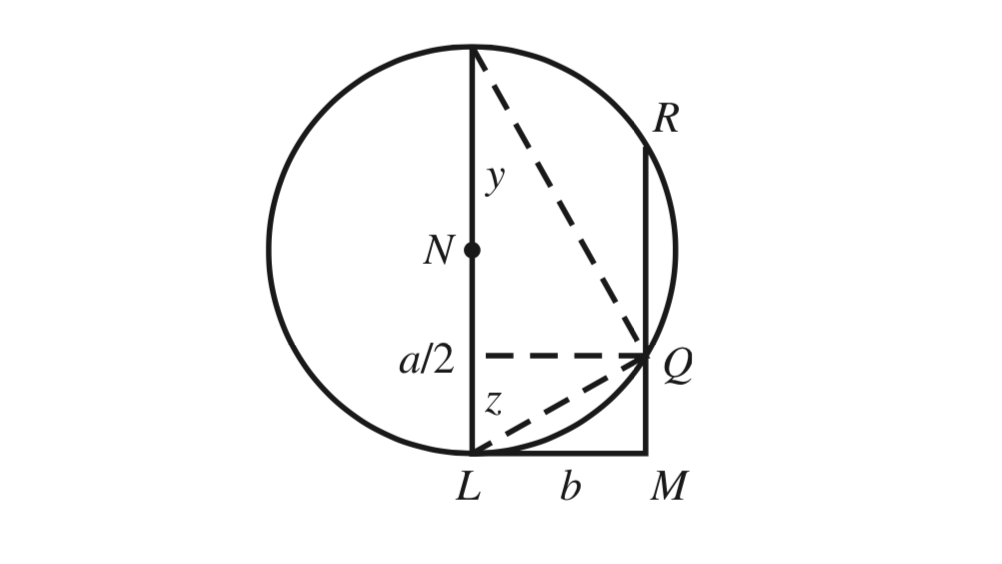
\includegraphics[ width = .5\textwidth]{imgg8.png}
  \end{center}
  Cutting the circle in the points $Q$ and $R$. Prove that that the lengths 
  $MQ$ and $MR$ represent the two positive solutions to $x^2 = ax - b^2$\\

  \solution Like the hint suggests lets suppose that $y = KJ$ and $z = JL$
   such that $y + z = a$. By carpenter's lemma and $AA$ similarity we know that $\triangle QJL \sim \triangle QJQ \sim \triangle KQL$. By similarity we know that,
   \begin{align*}
     \frac{b}{z} &= \frac{y}{b},\\
     b^2 &= yz
   \end{align*}
   
\end{exercise}
\vspace{.5in}










\textbf{Perspective Problems}

\begin{exercise}{1} 
  \solution 
\end{exercise}
\vspace{.5in}


\begin{exercise}{2} 
  \solution 
\end{exercise}
\vspace{.5in}


\textbf{Projective Problems}

\begin{exercise}{1} 
  \solution 
\end{exercise}
\vspace{.5in}



\textbf{Reflection}
\begin{enumerate}
  \item
  \item 
\end{enumerate}





\end{document}